\section{Phase 1 - Planning and research phase}

After we had gotten in touch with Accenture and spoken with the supervisors and the product owner, the group had to make a few decisions regarding the direction of the project.

The first choice to make was to either build an AI for the vehicles from scratch or use the AI from the group prior. Building the AI from scratch ment that we could make an AI which integrated our system from the start, however with the time constraint of the project we decided that it would take less time to use the product from the group prior. In addition, our group had more prior experience with networking than with raspberry Pi and AI. We therefore chose to use the AI from the project prior. We also had to decide which technologies and programming languages to use.

In this phase we did not have access to the vehicle made by the prior bachelor group and neither the code. In addition there was a need for project planning and research before we could start developing our IoT-system. The topics needed to be researched was:

\begin{itemize}
\item Research what causes traffic jams and solutions to fix it.
\item Research IoT-systems and how they function with vehicles.
\item Research different planning methods that will fit our project
\end{itemize}
We also used the pre-project phase to get to know Accenture, their guidelines and their workspace since we were going to work a their office. 



\subsection{Choice of programming languages}
We chose to implement the client in Python and the server in C\#. The group before us had used Python for their Raspberry Pi vehicle, making Python a natural choice to extend the code from their project. Our group also had experience with networking in Python. Furthermore, the .NET ecosystem has well-developed solutions for creating IoT applications, microservices, and web applications \parencite{dotnet}. We had to write our server in C\#, to take advantage of these solutions. The server needed to be as efficient as possible, and C\# is also considered a fast programming language \parencite{csharp}. We also had some prior knowledge of coding in C\#.

\subsection{Internet of Things}

The Internet Of Things refers to physical objects that communicate using sensors, cameras, software, or other technologies connecting and exchanging data. This communication takes place over the internet or other communication forms. The number of connected IoT devices in the world is increasing, and it is becoming a big part of society \parencite{iot_analytics}. IoT has also been evolving in recent years due to other technologies becoming more accessible, such as machine learning and the 5G network.

IoT projects can, for instance, be applied in climate surveillance systems, energy, or transportation. In this thesis we will explore the possibilities of using IoT in transportation, more specifically in personal automobiles. The convergence of these fields is more commonly known as IoV, Internet of Vehicles. An IoV system is a distributed system for wireless communication and information exchange between vehicles through agreed-upon communication protocols \parencite{chinese_iov}. The system could potentially integrate functionality for dynamic information exchange, vehicle control and smart traffic management. In our thesis, we will explore these possibilities on a small scale.

\subsection{Preventing traffic congestions for a one-lane road}\label{sec:traffic_congestion}

Traffic congestion, also known as traffic jams, is when a long line of vehicles moves slowly or has stopped moving altogether. Traffic jams can create frustration and disrupt nearby local environments with sound and gas emissions \parencite{traffic_congestion_pollution}. Many factors can cause traffic congestion, such as:

poorly designed roads, not wide enough roads, traffic light patterns, and accidents \parencite{traffic_congestion}.

With this in mind, we started by focusing on a simple scenario: when a car drastically reduces its speed or completely stops on a single-lane road.

This scenario will lead to the vehicles behind needing to slow down drastically as well. This phenomenon is called traffic jam shockwave \parencite{traffic_shockwave}. To prevent this, we propose a solution where cars reduce their velocity before they reach the destination of where the shockwave started. For this to happen, a server could keep track of the cars' positions and send information to the vehicles behind, when required. 

We came up with an idea on how the server and cars should interact. First, the car would connect to the server and provide information about its current speed, weight, width, and length. The server would use this information to keep track of all the cars' positions on the road. The cars would send information to the server if their velocity changed. This message would trigger an event on the server where it would command all the cars behind to slow down accordingly. \figref{fig:diagramfirst} shows a flow chart of a potential simulation of this solution:

\begin{figure}[h!]
	\centering
	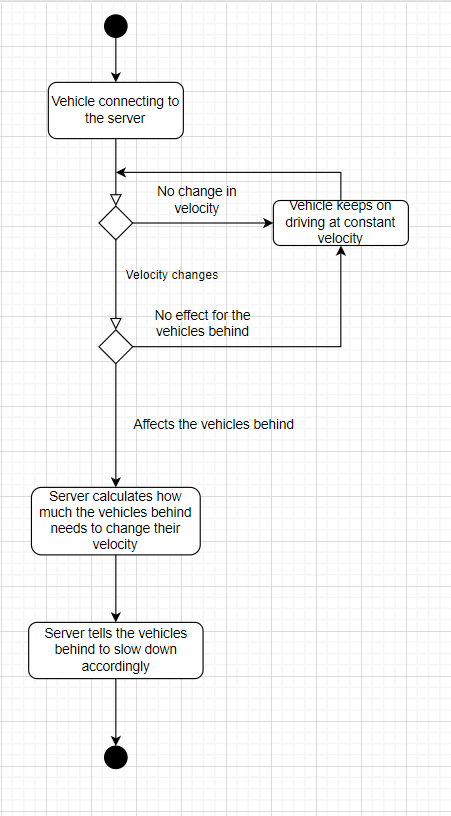
\includegraphics[width=0.9\linewidth]{figures/flow_diagram_first}
	\caption[Flow diagram server]{This figure shows the flow diagram of our first proposed solution. }
	\label{fig:diagramfirst}
\end{figure}
\clearpage
\section{Prioritization method}
The MoSCoW method is a prioritization technique used in project management. The word MoSCoW is an acronym where:

\begin{itemize}
	\item "Mo" stands for must-have and represents our project's most prioritized requirements. These are necessary for the success of our project.
	\item "S" stands for should have. Our project should include these requirements, but they are not mandatory.
	\item "Co" stands for could have. We want to include these requirements in our project but they are not prioritized.
	\item "W" stands for will not have this time. The requirements in the "W" section might be for a later group if someone wants to build on our project further.
\end{itemize}

<<<<<<< HEAD
Since we were unsure of how many use cases we could finish within the time frame of the project period, we thought a prioritization method was a good fit. \figref{fig:moscowmethod} shows our visualization of the Moscow method.
=======
Since we were unsure of how many features we could finish within the time frame of the project period, we thought a prioritization method was a good fit. Figure 3.2 shows our visualization of the Moscow method.
>>>>>>> 997a3d15b8ceb26c8c169ca7a83e895f9e750efc

\begin{figure}[h!]
	\centering
	\includegraphics[width=1\linewidth]{figures/MosCoW_method}
	\caption[MosCoW method]{Visualuzation MoSCoW method. Everything under "Mo" are requirements we must have in our project, under the "S" sections are features we should have. Under "Co" are features we should have, but are not necessary. Under "W" are features we will not have this time}
	\label{fig:moscowmethod}
\end{figure}


